% \documentclass[varwidth,10pt, border=10pt]{wlscirep}
\documentclass[varwidth, border=10pt, class=wlscirep, 10pt]{standalone}

\RequirePackage{helvet}
\RequirePackage{courier}

% border={10pt 5pt} % left/right bottom/top
% border={10pt 10pt 0pt 10pt} % left right bottom top


\usepackage{subcaption}
\usepackage[
    font=footnotesize,
    labelfont={bf,sf,footnotesize},
    labelsep=period,
    justification=raggedright
]{caption}
\usepackage{graphicx}

\begin{document}

\begin{figure}
    \centering

    \begin{subfigure}[b]{6cm}
        \centering
        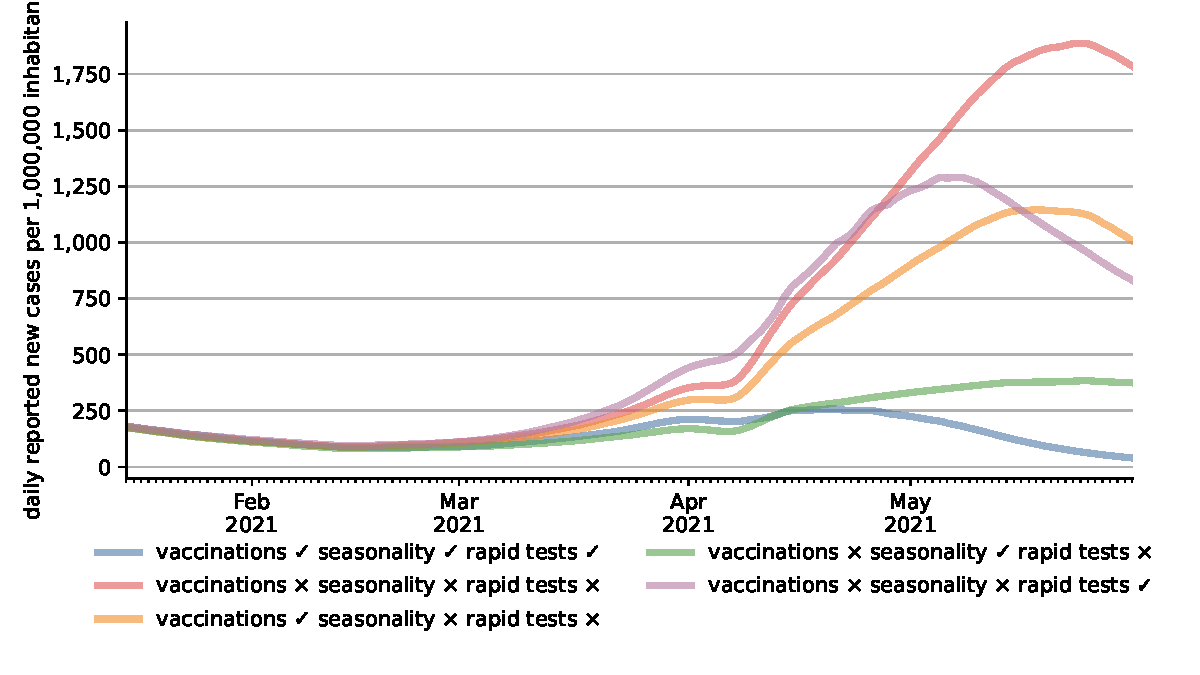
\includegraphics[width=5cm]{../figures/results/figures/scenario_comparisons/effect_of_channels_on_pessimistic_scenario/full_new_known_case}
        \caption{{Recorded cases: 2021 scenarios}}
        \label{fig:2021_scenarios_recorded}
    \end{subfigure}
    \hfill
    \begin{subfigure}[b]{6cm}
        \centering
        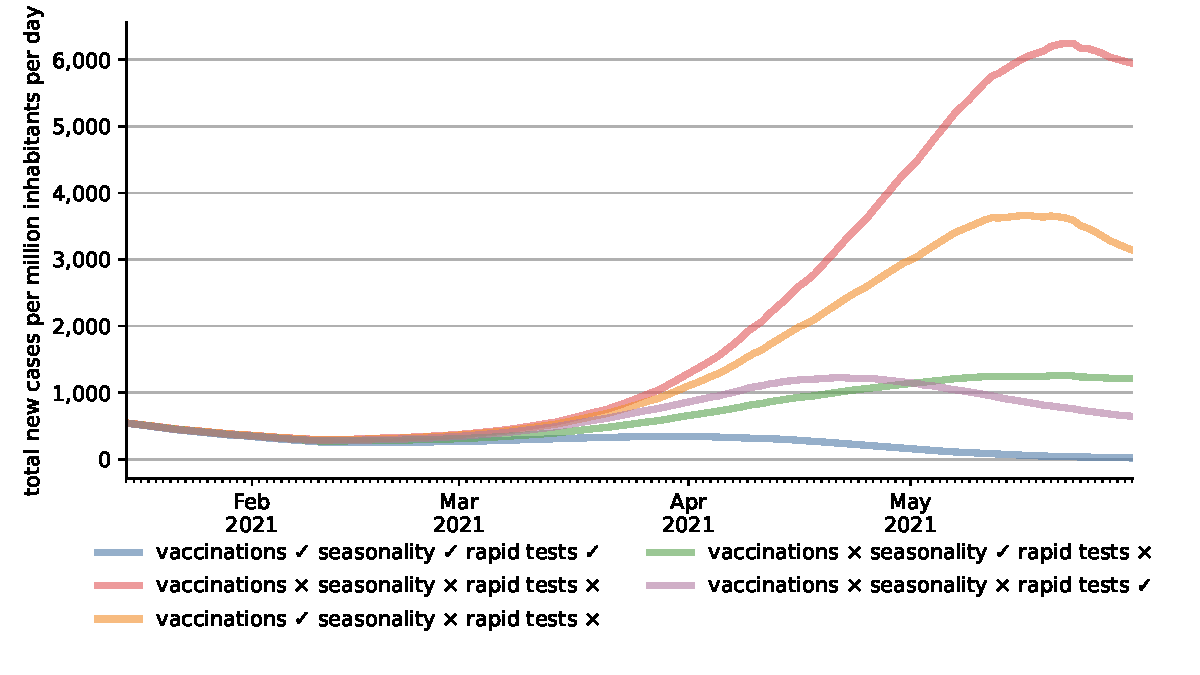
\includegraphics[width=5cm]{../figures/results/figures/scenario_comparisons/effect_of_channels_on_pessimistic_scenario/full_newly_infected}
        \caption{{Total cases: 2021 scenarios}}
        \label{fig:2021_scenarios_newly_infected}
    \end{subfigure}

    \begin{subfigure}[b]{6cm}
        \centering
        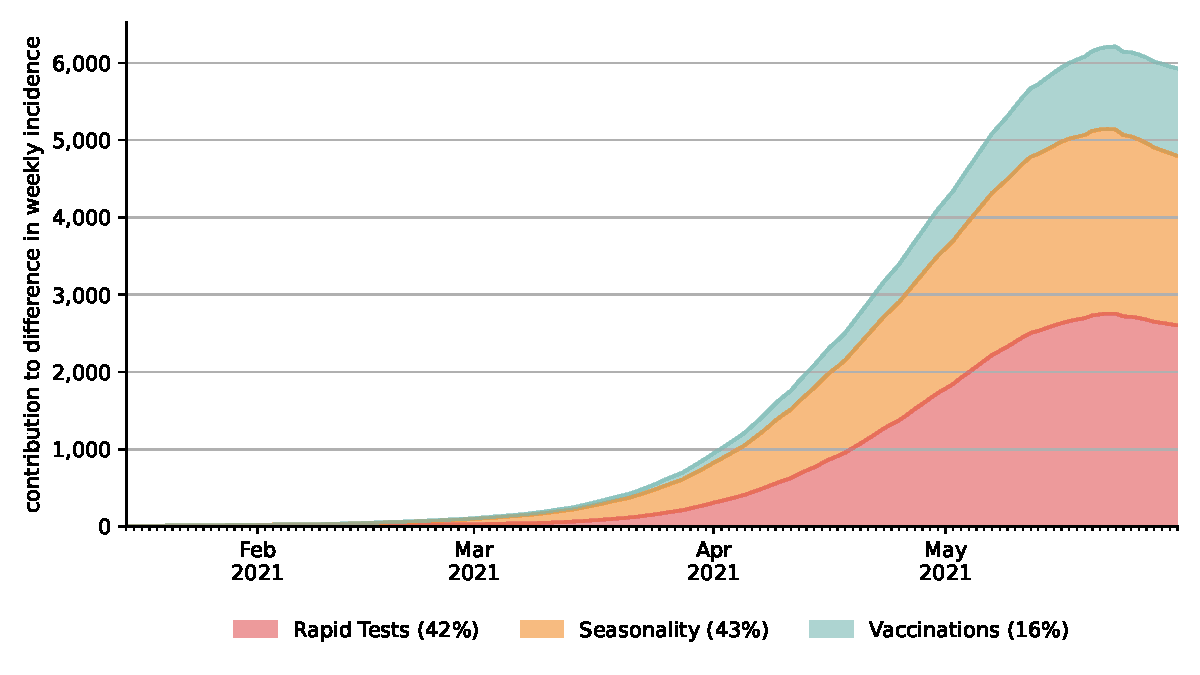
\includegraphics[width=5cm]{../figures/results/figures/full_decomposition_channels_area}
        \caption{Decomposition of the difference between the scenario without any of the
            three factors and the main scenario in
            Figure~3b.}
        \label{fig:2021_scenarios_decomposition}
    \end{subfigure}
    \hfill
    \begin{subfigure}[b]{6cm}
        \centering
        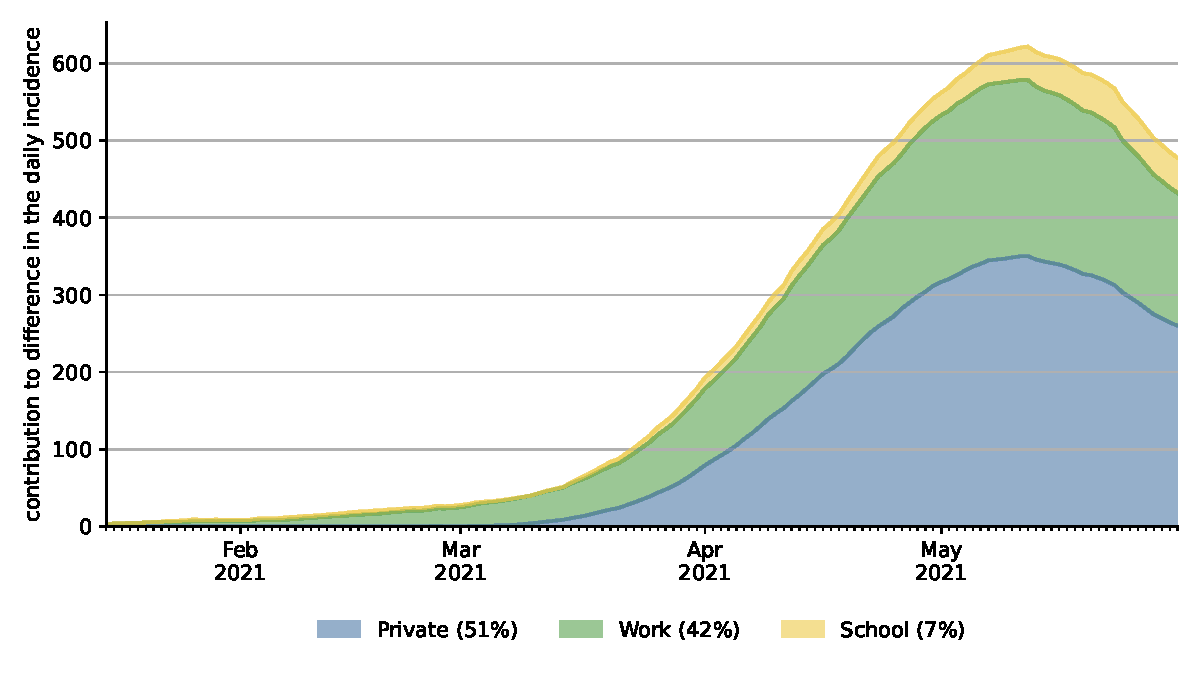
\includegraphics[width=5cm]{../figures/results/figures/full_decomposition_rapid_tests_area}
        \caption{Decomposition of the difference between the scenario without rapid
            tests and the main scenario in
            Figure~3b.}
        \label{fig:2021_scenarios_decomposition_tests}
    \end{subfigure}
\end{figure}

\end{document}
